% ============================================================
% Bai bao SSRC (IEEEtran) - tieng Viet - ban v2
% "Phat hien phuong tien giao thong Viet Nam bang YOLOv8s ..."
% BIEN DICH: XeLaTeX (Overleaf: Menu -> Compiler -> XeLaTeX)
% Thu muc can upload: main.tex + figures/ (3 anh PNG)
% ============================================================
\documentclass[10pt,journal,a4paper]{IEEEtran}

\usepackage{fontspec}
\setmainfont{texgyretermes}[Extension=.otf,UprightFont=*-regular,BoldFont=*-bold,ItalicFont=*-italic,BoldItalicFont=*-bolditalic]
\usepackage{amsmath,amssymb}
\usepackage{graphicx}
\usepackage{booktabs}
\usepackage{array}
\usepackage{url}
\Urlmuskip=0mu plus 1mu\relax
\graphicspath{{figures/}{./}}  % anh dat trong thu muc figures/ HOAC ngay thu muc goc deu duoc

\renewcommand{\figurename}{Hình}
\renewcommand{\tablename}{Bảng}
\renewcommand{\refname}{Tài liệu tham khảo}
\newcommand{\clspw}{\texttt{cls\_pw}}

\begin{document}

\title{Phát hiện phương tiện giao thông Việt Nam bằng YOLOv8s: so sánh với Faster R-CNN trong miền và ngoài miền trên dữ liệu chia theo video}

\author{Phạm Minh Hùng, Đặng Xuân Đức và Lê Thị Vĩnh Thanh$^{*}$\\
Tác giả liên hệ: \texttt{lethivinhthanh@iuh.edu.vn}}

\markboth{Student Scientific Research Communication, Volume II, 2026}{Student Scientific Research Communication, Volume II, 2026}
\maketitle

% ------------------------------------------------------------
\begin{abstract}
Vietnamese traffic data come from many cameras, and frames from the same video are nearly identical, so the evaluation of vehicle detectors is easily optimistic. This paper compares the one-stage detector YOLOv8s (11.1 million parameters) with the two-stage detector Faster R-CNN ResNet50-FPN (41.4 million parameters) on data split by video. Five public sources are merged into the V5+ set of 10,203 images with four classes (motorcycle, car, bus, truck). An additional audit shows that every validation image shares a camera scene with the training set, so the video-level split protects only the 1,500-image test set, whose two daytime cameras do not appear in training. Both detectors are trained on the same training set and evaluated with the same tool (pycocotools, up to 300 boxes per image). On the test set, Faster R-CNN reaches an mAP@0.5 of 0.7916 versus 0.7513 for the class-weighted YOLOv8s chosen as our final model (YOLOv8s-CW), a gap of 4.03 points (bootstrap 95\% CI [+2.95, +4.97]), whereas YOLOv8s has about 4.9 times lower per-image latency at the same FP32 precision. On the out-of-domain aerial-view set, YOLOv8s-CW has the higher mAP@0.5 (0.5991 versus 0.5640 on validation; 0.5759 versus 0.5242 on the small test split, where the difference is not significant), while Faster R-CNN has the higher mAP@0.5:0.95. The two detectors therefore trade accuracy for speed rather than one dominating the other, and the comparison is between models of different sizes. A controlled comparison with three seeds per condition shows that class weighting has only a negligible effect: fine-tuning from the same baseline gives a mean mAP@0.5 of 0.8008 with class weights and 0.8003 without them (Ultralytics), with per-seed differences between $-0.04$ and $+0.29$ points, whereas the extra fine-tuning itself adds about 1.1 points. A small-object head, a higher input resolution and a resolution curriculum do not improve the in-domain results either. Apart from the class-weighting experiment, each configuration was trained once and the final configuration was chosen after inspecting the test results, so the conclusions are preliminary evidence.
\end{abstract}

\renewcommand{\abstractname}{Tóm tắt}
\begin{abstract}
Dữ liệu phương tiện giao thông Việt Nam đến từ nhiều camera, và các khung hình cùng video gần như giống hệt nhau, nên việc đánh giá mô hình phát hiện dễ lạc quan. Bài báo so sánh bộ phát hiện một giai đoạn YOLOv8s (11,1 triệu tham số) với bộ phát hiện hai giai đoạn Faster R-CNN ResNet50-FPN (41,4 triệu tham số) trên dữ liệu được chia tập theo video. Chúng tôi hợp nhất năm nguồn công khai thành bộ V5+ gồm 10.203 ảnh với bốn lớp (xe máy, ô tô, xe buýt, xe tải). Kiểm tra bổ sung cho thấy mọi ảnh xác thực đều chung khung cảnh camera với tập huấn luyện, nên cách chia theo video chỉ bảo vệ được tập kiểm thử 1.500 ảnh, gồm hai camera ban ngày không xuất hiện trong huấn luyện. Hai mô hình được huấn luyện trên cùng tập huấn luyện và đánh giá bằng cùng một công cụ (pycocotools, tối đa 300 hộp mỗi ảnh). Trên tập kiểm thử, Faster R-CNN đạt mAP@0,5 là 0,7916, cao hơn YOLOv8s có trọng số lớp được chọn làm mô hình cuối (YOLOv8s-CW, 0,7513) 4,03 điểm (khoảng tin cậy 95\% bootstrap [+2,95; +4,97]), trong khi độ trễ mỗi ảnh của YOLOv8s thấp hơn khoảng 4,9 lần ở cùng FP32. Trên bộ ảnh góc nhìn trên cao ngoài miền, YOLOv8s-CW có mAP@0,5 cao hơn (0,5991 so với 0,5640 trên tập xác thực; 0,5759 so với 0,5242 trên tập kiểm thử nhỏ, nơi chênh lệch chưa có ý nghĩa thống kê), còn Faster R-CNN có mAP@0,5:0,95 cao hơn. Như vậy hai mô hình đánh đổi độ chính xác lấy tốc độ chứ không mô hình nào vượt trội hoàn toàn, và đây là so sánh giữa hai mô hình khác cỡ. Thí nghiệm đối chứng với ba hạt giống cho mỗi điều kiện cho thấy trọng số lớp chỉ có tác dụng không đáng kể: tinh chỉnh từ cùng mô hình cơ sở đạt mAP@0,5 trung bình 0,8008 khi có trọng số lớp và 0,8003 khi không có (Ultralytics), chênh lệch theo từng hạt giống từ $-0{,}04$ đến $+0{,}29$ điểm, trong khi riêng việc tinh chỉnh thêm đã tăng khoảng 1,1 điểm. Đầu phát hiện vật nhỏ, tăng độ phân giải và lộ trình độ phân giải cũng không cải thiện kết quả trong miền. Trừ thí nghiệm trọng số lớp, mỗi cấu hình chỉ được huấn luyện một lần và cấu hình cuối được chọn sau khi xem kết quả kiểm thử, nên các kết luận là bằng chứng sơ bộ.
\end{abstract}

\begin{IEEEkeywords}
Object detection, YOLOv8, Faster R-CNN, data leakage, vehicle detection, out-of-domain evaluation, class imbalance.
\end{IEEEkeywords}

\renewcommand{\IEEEkeywordsname}{Từ khóa}
\begin{IEEEkeywords}
Phát hiện đối tượng; YOLOv8; Faster R-CNN; rò rỉ dữ liệu; phương tiện giao thông; đánh giá ngoài miền; mất cân bằng lớp.
\end{IEEEkeywords}

% ============================================================
\section{Giới thiệu}
\IEEEPARstart{H}{ệ} thống camera giám sát giao thông tại các đô thị Việt Nam tạo ra lượng lớn hình ảnh có thể dùng để thống kê cơ cấu phương tiện, hỗ trợ quy hoạch và điều phối tín hiệu. Bài toán cốt lõi là phát hiện đối tượng đa lớp: xác định đồng thời vị trí và nhãn lớp của từng phương tiện trong khung hình. Các bộ phát hiện dựa trên mạng nơ-ron tích chập như YOLO~\cite{yolo} và Faster R-CNN~\cite{frcnn} thực hiện được cả hai yêu cầu này.

Dữ liệu giao thông Việt Nam có ba đặc điểm gây khó cho việc đánh giá. Thứ nhất, dữ liệu công khai (chủ yếu trên Roboflow Universe) đến từ nhiều camera với quy ước nhãn khác nhau, nên phải chuẩn hóa nhãn trước khi dùng chung. Thứ hai, các khung hình lấy từ cùng một video gần như giống hệt nhau. Nếu chia tập huấn luyện và kiểm thử theo khung hình, mô hình có thể ``ghi nhớ cảnh'' thay vì học khái niệm phương tiện, làm kết quả đánh giá lạc quan. Các phiên bản dữ liệu đầu của đề tài (V1--V4) chia theo khung hình nên có nguy cơ này; từ phiên bản V5, chúng tôi chuyển sang chia theo video. Thứ ba, phân bố lớp rất lệch: trên toàn bộ dữ liệu của chúng tôi, xe máy chiếm khoảng 69\% số hộp giới hạn (bounding box), ô tô 19\%, xe tải 9\% và xe buýt 3\%, nên độ chính xác trung bình trên các lớp (mean Average Precision, mAP) dễ che khuất chất lượng của các lớp thiểu số.

\textbf{Khoảng trống.} Các công trình trên dữ liệu Việt Nam mà chúng tôi tiếp cận được tập trung vào xây dựng bộ dữ liệu hoặc ứng dụng đếm, theo vết. Trinh và Nguyen~\cite{trinh} xây dựng bộ UIT-VinaDeveS22 từ sáu video camera, tách tập kiểm thử theo video có khung cảnh khác hẳn tập huấn luyện nhưng lấy tập xác thực từ cùng video với tập huấn luyện, và so sánh các bộ phát hiện một giai đoạn (YOLOX, YOLOF, RetinaNet, YOLACT) trong miền. Dinh và cộng sự~\cite{dinh} xây dựng hệ thống đếm phương tiện trên thiết bị biên với bộ dữ liệu VDD của Việt Nam, còn Vuong và cộng sự~\cite{vuong} dùng YOLOv4 và SORT để theo vết và ước lượng tốc độ phương tiện từ camera cố định ở Hà Nội. Theo những gì chúng tôi đọc được, các công trình này chưa đồng thời: (i) kiểm tra rò rỉ ở mức camera và nêu giới hạn của việc chia tập; (ii) so sánh bộ phát hiện một giai đoạn với hai giai đoạn bằng cùng công cụ đánh giá; (iii) đánh giá ngoài miền huấn luyện; (iv) báo cáo cả các cải tiến không hiệu quả kèm đối chứng. Chúng tôi không đề xuất một kiến trúc hay hàm mất mát mới; đóng góp của bài là một đánh giá có phương pháp và minh bạch về phạm vi.

\textbf{Đóng góp.} Bài báo có bốn đóng góp:
\begin{enumerate}
\item Hợp nhất năm nguồn công khai thành bộ V5+ gồm 10.203 ảnh theo lược đồ nhãn (schema) bốn lớp, chia tập theo video, kèm kiểm tra toàn vẹn nhãn và kiểm tra trùng khung cảnh camera giữa các tập. Chúng tôi nêu rõ phạm vi và giới hạn của kiểm tra này (Mục~\ref{sec:data}).
\item So sánh YOLOv8s với Faster R-CNN ResNet50-FPN huấn luyện trên cùng tập V5+ và đánh giá bằng cùng công cụ, về độ chính xác (kể cả theo từng lớp, kèm khoảng tin cậy bootstrap), số tham số và tốc độ, trong và ngoài miền.
\item Đánh giá ngoài miền trên bộ ảnh góc nhìn trên cao (VN Aerial) và báo cáo các cải tiến không hiệu quả (đầu phát hiện P2, tăng độ phân giải, lộ trình độ phân giải, thêm nhãn giả).
\item Khảo sát tham số trọng số lớp \clspw{} có sẵn trong Ultralytics bằng đối chứng $\clspw = 0$ và 0,5 với ba hạt giống, cùng điểm khởi đầu và cùng siêu tham số, cho thấy trọng số lớp chỉ tạo khác biệt dưới 0,3 điểm, nhỏ so với tác dụng của việc tinh chỉnh thêm.
\end{enumerate}

% ============================================================
\section{Công trình liên quan}
\subsection{Phát hiện đối tượng}
Mạng nơ-ron tích chập học đặc trưng trực tiếp từ ảnh thay cho các bộ mô tả thủ công. Mạng phần dư ResNet~\cite{resnet} dùng kết nối tắt để huấn luyện mạng sâu mà không suy biến gradient và thường là xương sống (backbone) của các bộ phát hiện; mạng kim tự tháp đặc trưng FPN~\cite{fpn} kết hợp đặc trưng nhiều tỷ lệ để phát hiện vật có kích thước khác nhau.

Faster R-CNN~\cite{frcnn} là đại diện của hướng hai giai đoạn: mạng đề xuất vùng (RPN) dùng chung đặc trưng tích chập với mạng phát hiện sinh các ứng viên, sau đó đầu phân loại và hồi quy tinh chỉnh từng ứng viên. Hướng một giai đoạn bỏ bước đề xuất vùng: YOLO~\cite{yolo} xử lý toàn ảnh trong một lượt và dự đoán trực tiếp hộp và lớp, còn SSD~\cite{ssd} dự đoán trên các hộp mặc định ở nhiều độ phân giải đặc trưng. Hai hướng này đánh đổi tốc độ lấy độ chính xác theo cách khác nhau, nên chúng tôi so sánh cả hai trên cùng dữ liệu.

YOLOv8 là phiên bản do Ultralytics duy trì~\cite{ultra}, có đầu tách nhánh phân loại và hồi quy, thiết kế không neo (anchor-free), và hàm mất mát kết hợp mất mát hộp với Distribution Focal Loss (DFL)~\cite{gfl}. Chúng tôi chọn biến thể small (YOLOv8s) làm mô hình chính vì cân bằng giữa tốc độ và độ chính xác, đồng thời vừa với bộ nhớ 12~GB của GPU thí nghiệm; Faster R-CNN ResNet50-FPN là mô hình đối chứng.

\subsection{Mất cân bằng lớp trong phát hiện đối tượng}
Các hướng chính là đặt lại trọng số mất mát và lấy mẫu lại. Class-balanced loss gán trọng số theo số mẫu hiệu dụng của mỗi lớp~\cite{cbloss}; focal loss giảm đóng góp của mẫu dễ~\cite{focal}. Với phân bố đuôi dài trên LVIS, Equalization Loss~\cite{eql} và Seesaw Loss~\cite{seesaw} điều chỉnh gradient của các lớp hiếm. Phan và Yamamoto~\cite{phan} thử nghiệm các biến thể cross-entropy có trọng số trên BDD100K~\cite{bdd}, tập dữ liệu lái xe có ô tô chiếm ưu thế. Ngược lại, Crasto~\cite{crasto} báo cáo rằng lấy mẫu và đặt lại trọng số mất mát không mang lại hiệu quả tương ứng cho YOLOv5 trên COCO-ZIPF, một tập con 10 lớp có phân bố đuôi dài của COCO, trong khi tăng cường mosaic và mixup cải thiện mAP rõ rệt. Vì hiệu quả của đặt lại trọng số với bộ phát hiện một giai đoạn chưa chắc chắn, chúng tôi thử một cấu hình trọng số lớp cho YOLOv8 kèm đối chứng không trọng số.

\subsection{Dữ liệu giao thông}
Các bộ dữ liệu như UA-DETRAC~\cite{detrac} và BDD100K~\cite{bdd} được dùng rộng rãi cho phương tiện. Cả hai được thu thập ở nước ngoài, với tỷ lệ xe máy thấp và tổ chức giao thông khác Việt Nam, nên số liệu trên các bộ này không thay thế được đánh giá trên dữ liệu trong nước. COCO~\cite{coco} chủ yếu đóng vai trò nguồn trọng số tiền huấn luyện trong học chuyển giao. Dữ liệu công khai về phương tiện Việt Nam chủ yếu được phát hành trên Roboflow Universe từ nhiều camera với quy ước nhãn khác nhau, vì vậy cần chuẩn hóa nhãn và kiểm soát cách chia tập trước khi huấn luyện.

\subsection{Rò rỉ dữ liệu khi chia tập theo khung hình}
Camera cố định quay 25--30 khung hình mỗi giây; hai khung hình liên tiếp có nền, vạch kẻ và ánh sáng gần như giống nhau, chỉ khác vị trí phương tiện vài điểm ảnh. Chia ngẫu nhiên theo khung hình đặt các bản sao gần như y hệt vào cả tập huấn luyện lẫn kiểm thử, nên điểm kiểm thử đo khả năng ``nhớ cảnh'' hơn là khả năng khái quát. Chia theo video là bước kiểm soát cần thiết, nhưng chưa đủ: hai video khác nhau vẫn có thể quay cùng một camera và cùng cảnh, nên đánh giá độc lập thực sự đòi hỏi gom mọi video của cùng camera vào một tập. Nhận định này là kết luận từ kiểm tra dữ liệu của chúng tôi (Mục~\ref{sec:data}) chứ không dẫn từ một công trình cụ thể.

% ============================================================
\section{Dữ liệu}\label{sec:data}
\subsection{Nguồn dữ liệu và lược đồ nhãn bốn lớp}
Bộ V5+ hợp nhất năm nguồn công khai, đều theo giấy phép CC BY 4.0 trên Roboflow Universe (Bảng~\ref{tab:sources}). Nhãn của mọi nguồn được quy đổi về bốn lớp: xe máy (motorcycle), ô tô con (car), xe buýt (bus) và xe tải (truck, gồm cả container). Các lớp khác như xe đạp, xe ba gác, xe van hoặc người bị loại bỏ thay vì gộp sang lớp gần nhất, nhằm tránh học nhầm hình dáng. Ảnh chỉ còn nhãn bị loại được giữ lại như ảnh nền. Tổng cộng có 10.203 ảnh từ 368 camera hoặc bối cảnh, chứa 87.460 hộp giới hạn. Theo cách phân nhóm kích thước của COCO~\cite{coco}, khoảng 16\% số hộp thuộc nhóm nhỏ, 67\% nhóm vừa và 17\% nhóm lớn.

\begin{table}[!t]
\centering
\caption{Các nguồn dữ liệu của bộ V5+ (số ảnh sau lấy mẫu, số camera hoặc bối cảnh, số hộp theo lớp)}
\label{tab:sources}
\resizebox{\columnwidth}{!}{%
\begin{tabular}{lrrrrrr}
\toprule
Nguồn & Ảnh & Camera & Xe máy & Ô tô & Xe buýt & Xe tải\\
\midrule
SOICT 2024 (ngày, TP.HCM) & 3.379 & 7 & 49.691 & 11.260 & 1.779 & 4.605\\
SOICT Night (đêm, TP.HCM) & 1.385 & 3 & 4.751 & 2.578 & 748 & 844\\
Vehicle Vietnam-CanTho & 725 & 4 & 2.152 & 1.710 & 19 & 140\\
Vietnamese Vehicle v3 & 310 & $\sim$310 & 471 & 570 & 68 & 361\\
Vietnam Vehicles v10 & 4.404 & 44 & 3.336 & 265 & 253 & 1.859\\
\midrule
\textbf{Tổng V5+} & \textbf{10.203} & \textbf{368} & \textbf{60.401} & \textbf{16.383} & \textbf{2.867} & \textbf{7.809}\\
Tỷ lệ số hộp & & & 69\% & 19\% & 3\% & 9\%\\
\bottomrule
\end{tabular}}
\end{table}

Phân bố lớp của riêng tập huấn luyện khác với toàn bộ V5+, vì tập kiểm thử (49.446 hộp) chiếm hơn một nửa số hộp. Tập huấn luyện 7.237 ảnh có 25.994 hộp: 13.460 xe máy (51,8\%), 5.921 ô tô (22,8\%), 1.652 xe buýt (6,4\%) và 4.961 xe tải (19,1\%). Trọng số lớp ở Mục~\ref{sec:clspw} được Ultralytics tính từ các con số này, sau khi bỏ một số nhãn trùng lặp.

\subsection{Chia tập và kiểm soát rò rỉ}
Tập huấn luyện gồm 7.237 ảnh (gồm toàn bộ 4.404 ảnh của Vietnam Vehicles v10), tập xác thực (validation) 1.466 ảnh và tập kiểm thử 1.500 ảnh. Tập kiểm thử chỉ gồm hai camera ban ngày của SOICT 2024 (\texttt{cam\_09} với 1.000 ảnh và \texttt{cam\_10} với 500 ảnh). Video ngày được lấy mẫu mỗi 5 khung hình, video đêm mỗi 10 khung hình; ảnh snapshot được giữ nguyên.

Chúng tôi chia theo \texttt{video\_id} suy ra từ tên tệp; với ảnh snapshot của Vietnam Vehicles v10, mỗi ảnh được coi là một video vì tên tệp không chứa mã camera. Kiểm tra theo quy tắc này không tìm thấy giao nhau giữa các tập, nhưng kiểm tra bổ sung cho thấy quy tắc này chưa đủ. Thứ nhất, 466 ảnh xác thực của Cần Thơ thuộc cùng camera với ảnh Cần Thơ trong tập huấn luyện, và có 102 cặp ảnh gần trùng giữa tập huấn luyện và tập xác thực. Thứ hai, khi so trực quan khung hình của từng camera SOICT, ba camera của SOICT Night (đều thuộc tập huấn luyện) quay cùng khung cảnh với camera ban ngày: \texttt{cam\_03} với \texttt{cam\_01} và \texttt{cam\_02}, \texttt{cam\_05} với \texttt{cam\_04}, và \texttt{cam\_08} với \texttt{cam\_07}. Vì \texttt{cam\_07} là nguồn của 1.000 ảnh xác thực còn lại, toàn bộ 1.466 ảnh xác thực đều có khung cảnh đã xuất hiện trong tập huấn luyện. Không camera đêm nào trùng khung cảnh với \texttt{cam\_09} hoặc \texttt{cam\_10}, nên hai camera kiểm thử không xuất hiện trong tập huấn luyện và tập xác thực theo kiểm tra này. Vì vậy chúng tôi chỉ khẳng định rò rỉ được giảm thiểu, chưa được loại bỏ: việc chọn điểm lưu (checkpoint) theo tập xác thực có thể lạc quan, và con số trên tập kiểm thử đáng tin hơn con số trên tập xác thực.

Để đo khả năng tổng quát hóa ngoài miền, chúng tôi dùng bộ VN Aerial gồm 486 ảnh xác thực và 149 ảnh kiểm thử chụp từ góc nhìn trên cao; so khớp MD5 xác nhận không có ảnh nào trùng với V5+. VN Aerial chỉ dùng để đánh giá, không tham gia huấn luyện.

% ============================================================
\section{Phương pháp}
\subsection{Mô hình cơ sở}
Mô hình cơ sở là YOLOv8s khởi tạo từ trọng số COCO~\cite{coco}, huấn luyện tối đa 40 epoch ở độ phân giải $960 \times 960$, batch 6, tốc độ học ban đầu 0,005 với lịch cosine và mixup 0,1~\cite{mixup}. Điểm lưu tốt nhất được chọn theo chỉ số fitness của Ultralytics trên tập xác thực (chủ yếu dựa trên mAP@0,5:0,95) và đạt ở epoch 26. Đây là điểm xuất phát chung cho các cải tiến bên dưới. Chúng tôi gọi mô hình này là cơ sở V5+.

Bảng~\ref{tab:config} tóm tắt khởi tạo, số epoch thực chạy, kích thước ảnh, batch và tốc độ học của mọi cấu hình. Mọi lượt chạy YOLO chỉ định tường minh bộ tối ưu SGD (động lượng 0,937) trong tệp cấu hình, nên tốc độ học trong Bảng~\ref{tab:config} là giá trị thực được dùng. Các siêu tham số còn lại (hộp 7,5, phân loại 0,5, DFL 1,5, lật ngang 0,5, mosaic 1,0, ba epoch khởi động) giữ mặc định của Ultralytics và giống nhau ở mọi cấu hình YOLO.

\begin{table}[!t]
\centering
\caption{Cấu hình huấn luyện của các mô hình (epoch là số epoch thực chạy; *phần trọng số COCO tương thích; $\times$2 là tích lũy gradient hai bước)}
\label{tab:config}
\resizebox{\columnwidth}{!}{%
\begin{tabular}{llcccc}
\toprule
Cấu hình & Khởi tạo & Epoch & Ảnh & Batch & lr0\\
\midrule
Cơ sở V5+ & COCO & 40 (tốt nhất 26) & 960 & 6 & 0,005\\
p4\_scale & Cơ sở V5+ & 28 & 960 & 6 & 0,0005\\
p4\_imgsz1280 & Cơ sở V5+ & 40 & 1.280 & 6 & 0,0005\\
r\_p2 & COCO* & 25 & 960 & 16 & 0,005\\
r\_progressive & COCO & 20 + 10 & 960 $\rightarrow$ 1.280 & 16 / 8 & 0,005 / 0,002\\
YOLOv8s-CW & Cơ sở V5+ & 10 (tốt nhất 2) & 960 & 16 & 0,001\\
Đối chứng $\clspw = 0$ ($\times$3) & Cơ sở V5+ & 10 & 960 & 16 & 0,001\\
Đối chứng $\clspw = 0{,}5$ ($\times$3) & Cơ sở V5+ & 10 & 960 & 16 & 0,001\\
Faster R-CNN & COCO & 8 (tốt nhất 8) & 800 / 1.333 & 4 ($\times$2) & 0,005\\
\bottomrule
\end{tabular}}
\end{table}

\subsection{Trọng số lớp trong mất mát phân loại}\label{sec:clspw}
Ultralytics (phiên bản 8.4.126) tính trọng số cho từng lớp từ số thực thể của lớp đó trong tập huấn luyện~\cite{ultraloss}. Gọi $n_c$ là số thực thể của lớp $c$ và $\gamma$ là tham số \clspw, trọng số được chuẩn hóa để trung bình bốn lớp bằng 1:
\begin{equation}
w_c = \frac{\left(\frac{1}{n_c}\right)^{\gamma}}{\frac{1}{4}\sum_{k=1}^{4}\left(\frac{1}{n_k}\right)^{\gamma}}, \qquad
\mathcal{L}_{\mathrm{cls}} = \sum_{c} w_c\, \ell_{\mathrm{BCE},c}
\label{eq:clspw}
\end{equation}

Chỉ mất mát phân loại (BCE) được nhân trọng số; mất mát hộp và DFL không đổi. Với $\gamma = 0{,}5$, bốn trọng số lần lượt là 0,571 (xe máy), 0,860 (ô tô), 1,629 (xe buýt) và 0,940 (xe tải). Mô hình có trọng số lớp, ký hiệu YOLOv8s-CW, được tinh chỉnh tối đa 15 epoch từ điểm lưu của cơ sở V5+ (khởi tạo ấm), tốc độ học 0,001, hệ số tốc độ học cuối 0,1, batch 16, hạt giống 0 và tắt mosaic ở 5 epoch cuối. Huấn luyện dừng sớm tại epoch 10 (patience 8); điểm lưu tốt nhất theo tập xác thực đạt ở epoch 2. Tham số \texttt{copy\_paste} bằng 0,3 ở cơ sở và 0 ở YOLOv8s-CW; theo mã nguồn Ultralytics 8.4.126 (lớp \texttt{CopyPaste} trong \texttt{ultralytics/data/augment.py}), phép tăng cường này trả nguyên nhãn khi ảnh không có nhãn đa giác, nên nó không có tác dụng với nhãn chỉ gồm hộp giới hạn của chúng tôi.

\textbf{Đối chứng trọng số lớp.} Để tách tác dụng của trọng số lớp khỏi tác dụng của việc tinh chỉnh thêm, chúng tôi chạy lại phép tinh chỉnh trên ở hai điều kiện $\clspw = 0$ và $\clspw = 0{,}5$, mỗi điều kiện với ba hạt giống (0, 1, 2). Mọi lượt có cùng điểm khởi đầu (cơ sở V5+), tốc độ học, batch, mixup, \texttt{copy\_paste} và \texttt{close\_mosaic} như YOLOv8s-CW, nhưng chạy cố định 10 epoch không dừng sớm để có cùng ngân sách; điểm lưu được chọn theo tập xác thực. YOLOv8s-CW là lượt chạy trước đó với lịch 15 epoch và dừng sớm, nên lịch tốc độ học của nó khác các lượt đối chứng.

\subsection{Các cấu hình đối chứng}
Để đặt YOLOv8s-CW trong bối cảnh, chúng tôi huấn luyện thêm bốn cấu hình YOLOv8s (Bảng~\ref{tab:config}): (i) p4\_scale, tăng cường không gian mạnh hơn (scale = 0,7, translate = 0,15), khởi tạo ấm từ cơ sở với tốc độ học 0,0005; (ii) p4\_imgsz1280, tăng độ phân giải lên 1.280, khởi tạo ấm từ cơ sở; (iii) r\_p2, thêm đầu phát hiện bước nhảy 4 (kiến trúc P2) cho vật nhỏ, khởi tạo từ phần trọng số COCO tương thích và huấn luyện 25 epoch; (iv) r\_progressive, lộ trình độ phân giải (curriculum) gồm 20 epoch ở 960 rồi 10 epoch ở 1.280, khởi tạo từ COCO. Như vậy ba cấu hình khởi tạo ấm có tổng ngân sách huấn luyện lớn hơn cơ sở, còn r\_p2 và r\_progressive có ít epoch hơn cơ sở.

Ngoài ra chúng tôi huấn luyện Faster R-CNN ResNet50-FPN của TorchVision~\cite{tv} khởi tạo từ COCO trên cùng tập huấn luyện V5+ làm mô hình đối chứng hai giai đoạn: 8 epoch, SGD (động lượng 0,9, Nesterov, weight decay 0,0005), batch 4 với tích lũy gradient hai bước, tốc độ học 0,005 với hai epoch khởi động tuyến tính rồi lịch cosine về 0, huấn luyện độ chính xác hỗn hợp, cạnh ngắn của ảnh 800 và cạnh dài tối đa 1.333, tăng cường lật ngang và màu sắc, hạt giống 42. Sau mỗi epoch, mô hình được đánh giá trên toàn bộ tập xác thực và điểm lưu có mAP@0,5 cao nhất được giữ lại; điểm lưu này đạt ở epoch 8. Mô hình có 41,4 triệu tham số, gấp khoảng 3,7 lần YOLOv8s (11,1 triệu). Khi suy luận để đánh giá, mô hình giữ tối đa 300 hộp mỗi ảnh với ngưỡng điểm 0,001 và NMS IoU 0,5, cùng giới hạn số hộp với YOLO; ảnh kiểm thử đông nhất có 64 hộp thực tế.

\subsection{Theo vết và đếm phương tiện}
Để dùng bộ phát hiện cho thống kê cơ cấu giao thông, chúng tôi ghép nó với bộ theo vết ByteTrack~\cite{bytetrack} (Hình~\ref{fig:pipeline}). ByteTrack liên kết các phát hiện giữa các khung hình bằng độ chồng lấp IoU, ghép trước các phát hiện có độ tin cậy cao rồi mới ghép các phát hiện độ tin cậy thấp với những vết chưa được gán, và dùng bộ lọc Kalman để dự đoán vị trí khi bị che ngắn. Đầu ra là một mã định danh (ID) bền vững cho mỗi phương tiện.

\begin{figure}[!t]
\centering
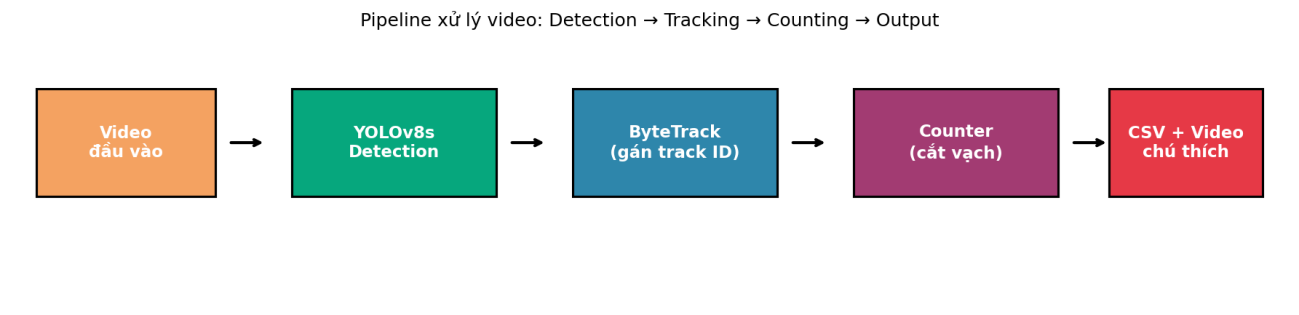
\includegraphics[width=\columnwidth]{fig1_pipeline.png}
\caption{Quy trình suy luận: YOLOv8s phát hiện phương tiện trên từng khung hình, ByteTrack gán ID theo vết, bộ đếm ghi nhận giao cắt với vạch ảo và xuất tệp CSV sự kiện cùng video chú thích.}
\label{fig:pipeline}
\end{figure}

Phép đếm dựa trên giao cắt đoạn thẳng. Người dùng đặt vạch ảo và chọn hướng đếm; lớp đếm hỗ trợ nhiều vạch, giao diện hiện cấu hình được một vạch. Với mỗi ID, hệ thống lưu tâm hộp ở khung hình trước; nếu đoạn nối tâm cũ với tâm mới cắt vạch, hệ thống ghi một sự kiện đếm gồm khung hình, tên vạch, hướng (xác định bằng dấu tích có hướng), ID và lớp. Mỗi cặp (vạch, ID) chỉ được đếm một lần, nên xe tấp vào lề rồi chạy ra không bị đếm hai lần. Kết quả xuất ra tệp CSV sự kiện và video chú thích.

\subsection{Chỉ số đánh giá}
Chúng tôi báo cáo Precision, Recall, mAP@0,5, mAP@0,5:0,95 và AP@0,5 theo từng lớp trên 1.500 ảnh kiểm thử, bằng hai cách. (a) So sánh các cấu hình YOLO với nhau dùng \texttt{model.val()} của Ultralytics (FP16, ngưỡng điểm 0,001, NMS IoU 0,7, tối đa 300 hộp); Precision và Recall là giá trị tại ngưỡng tin cậy cho F1 trung bình các lớp cao nhất, được Ultralytics chọn trên chính tập đang đánh giá. (b) So sánh YOLO với Faster R-CNN dùng pycocotools trên cùng tệp nhãn chuyển từ nhãn YOLO, cùng ngưỡng điểm 0,001 và tối đa 300 hộp mỗi ảnh; Precision và Recall của cách (b) được tính theo cùng định nghĩa tại IoU 0,5. Hai công cụ cho giá trị tuyệt đối khác nhau nên chúng tôi không so số giữa hai cách. Do tính ngẫu nhiên của suy luận FP16, chênh lệch dưới 0,003 giữa các lần đánh giá lại cùng một điểm lưu được coi là trùng khớp. Số TP, FP và FN theo lớp được đếm ở ngưỡng tin cậy 0,25, NMS IoU 0,7 và ghép hộp với IoU $\geq$ 0,5. Kích thước hộp theo chuẩn COCO~\cite{coco}: nhỏ ($< 32^2$ pixel), vừa ($32^2$--$96^2$) và lớn ($> 96^2$).

% ============================================================
\section{Kết quả thực nghiệm}\label{sec:results}
Các lượt huấn luyện YOLO, mọi phép đánh giá và đo tốc độ chạy trên một GPU NVIDIA RTX 3500 Ada Laptop 12~GB với Python 3.10. Cơ sở V5+, p4\_scale, p4\_imgsz1280, r\_p2 và r\_progressive được huấn luyện với PyTorch 2.5.1 và Ultralytics 8.4.142; YOLOv8s-CW và các lượt đối chứng được huấn luyện với PyTorch 2.7.1 và Ultralytics 8.4.126. Mọi phép đánh giá trong bài dùng cùng một môi trường: PyTorch 2.7.1, TorchVision 0.22.1 và Ultralytics 8.4.126. Riêng Faster R-CNN được huấn luyện trên GPU NVIDIA Tesla T4 (Google Colab) với Python 3.13, PyTorch 2.7.1 và TorchVision 0.22.1. Trừ thí nghiệm đối chứng trọng số lớp (ba hạt giống), mỗi cấu hình chỉ được huấn luyện một lần với một hạt giống ngẫu nhiên. Để ước lượng độ bất định do chọn ảnh kiểm thử, chúng tôi lấy mẫu có hoàn lại 1.500 ảnh kiểm thử 1.000 lần, tính mAP@0,5 của hai mô hình trên cùng mẫu và báo cáo khoảng tin cậy 95\% của hiệu số; khoảng này không phản ánh dao động giữa các lần huấn luyện. Chênh lệch giữa hai giá trị mAP hoặc AP được tính bằng điểm phần trăm (gọi tắt là điểm), ví dụ 0,7984 so với 0,7930 là 0,54 điểm.

\subsection{So sánh các cấu hình trên tập kiểm thử}
Bảng~\ref{tab:ultra} cho thấy, theo Ultralytics, YOLOv8s-CW đạt mAP@0,5 là 0,7984, hơn cơ sở V5+ 0,54 điểm và hơn p4\_scale 1,13 điểm. Tuy nhiên, khi lặp lại phép tinh chỉnh với ba hạt giống, điều kiện $\clspw = 0{,}5$ đạt trung bình $0{,}8008 \pm 0{,}0031$ và điều kiện $\clspw = 0$ đạt $0{,}8003 \pm 0{,}0042$: chênh 0,05 điểm, nhỏ hơn độ lệch giữa các hạt giống. Cả hai đều cao hơn cơ sở khoảng 0,8 điểm, nên mức tăng so với cơ sở chủ yếu đến từ việc tinh chỉnh thêm vài epoch với tốc độ học nhỏ chứ không phải từ trọng số lớp. Lượt $\clspw = 0{,}5$ với hạt giống 0 có cùng cấu hình và hạt giống với YOLOv8s-CW nhưng lịch 10 epoch, đạt 0,8031 so với 0,7984, cho thấy riêng việc đổi lịch học đã tạo chênh lệch cỡ nửa điểm. Các cấu hình P2, tăng độ phân giải và lộ trình độ phân giải đều thấp hơn cơ sở. Để tham chiếu, YOLOv8s COCO không huấn luyện lại chỉ đạt 0,4514 mAP@0,5.

Bảng~\ref{tab:coco} so sánh YOLO với Faster R-CNN bằng cùng pycocotools, cả hai huấn luyện trên V5+. Trên tập kiểm thử V5+, Faster R-CNN đạt 0,7916 mAP@0,5 và 0,4244 mAP@0,5:0,95, cao hơn YOLOv8s-CW (0,7513 và 0,4029) 4,03 điểm mAP@0,5 (khoảng tin cậy 95\% bootstrap [+2,95; +4,97]) và cao hơn trung bình ba hạt giống của $\clspw = 0{,}5$ 3,30 điểm ([+2,21; +4,17]). Tại ngưỡng cho F1 cao nhất, Faster R-CNN có Precision 0,7491 và Recall 0,7267, so với 0,7542 và 0,7365 của YOLOv8s-CW. Theo cùng công cụ, hiệu số giữa YOLOv8s-CW và cơ sở là +0,51 điểm ([$-0{,}05$; +1,09], khoảng tin cậy chứa 0), nên mức tăng này chưa có ý nghĩa thống kê. Trong thí nghiệm đối chứng, trung bình ba hạt giống của $\clspw = 0{,}5$ cao hơn $\clspw = 0$ 0,13 điểm ([+0,03; +0,22]); khoảng này chỉ tính dao động do chọn ảnh kiểm thử, còn chênh lệch theo từng hạt giống là $-0{,}04$, +0,29, +0,13 điểm. Riêng việc tinh chỉnh thêm ($\clspw = 0$) đã hơn cơ sở 1,12 điểm ([+0,75; +1,51]). Trên VN Aerial, thứ tự đảo lại ở mAP@0,5: YOLOv8s-CW đạt 0,5991 trên tập xác thực và 0,5759 trên tập kiểm thử, so với 0,5640 và 0,5242 của Faster R-CNN (hiệu số +3,51 điểm, [+1,50; +5,17], và +5,17 điểm, [$-0{,}85$; +11,66]; tập kiểm thử chỉ có 149 ảnh nên khoảng tin cậy chứa 0). Ngược lại, ở mAP@0,5:0,95 Faster R-CNN cao hơn YOLOv8s-CW trên cả hai tập VN Aerial (0,2910 và 0,2580 so với 0,2805 và 0,2504): ngoài miền, Faster R-CNN tìm được ít đối tượng hơn ở IoU 0,5 nhưng các hộp nó tìm được khớp chặt hơn.

\begin{table}[!t]
\centering
\caption{Kết quả trên tập kiểm thử V5+ (1.500 ảnh), đánh giá bằng \texttt{model.val()} của Ultralytics}
\label{tab:ultra}
\resizebox{\columnwidth}{!}{%
\begin{tabular}{lcccc}
\toprule
Mô hình & mAP@0,5 & mAP@0,5:0,95 & P & R\\
\midrule
Cơ sở V5+ & 0,7930 & 0,4279 & 0,7643 & 0,7283\\
p4\_scale & 0,7871 & 0,4236 & 0,7581 & 0,7327\\
p4\_imgsz1280 & 0,7741 & 0,4175 & 0,7285 & 0,7427\\
r\_p2 & 0,7528 & 0,3944 & 0,7409 & 0,7075\\
r\_progressive & 0,7710 & 0,4148 & 0,7405 & 0,7211\\
YOLOv8s-CW & 0,7984 & 0,4283 & 0,7648 & 0,7445\\
$\clspw = 0$ (TB 3 lần) & $0{,}8003 \pm 0{,}0042$ & 0,4301 & 0,7701 & 0,7377\\
$\clspw = 0{,}5$ (TB 3 lần) & $0{,}8008 \pm 0{,}0031$ & 0,4304 & 0,7698 & 0,7370\\
Faster R-CNN R50-FPN & 0,7945 & 0,4247 & 0,7504 & 0,7241\\
\bottomrule
\end{tabular}}
\end{table}

\begin{table}[!t]
\centering
\caption{Đánh giá thống nhất bằng pycocotools (cùng tệp nhãn, ngưỡng điểm 0,001, tối đa 300 hộp mỗi ảnh); Aerial là mAP@0,5 trên VN Aerial}
\label{tab:coco}
\resizebox{\columnwidth}{!}{%
\begin{tabular}{lcccc}
\toprule
 & \multicolumn{2}{c}{V5+ kiểm thử} & \multicolumn{2}{c}{Aerial}\\
\cmidrule(lr){2-3}\cmidrule(lr){4-5}
Mô hình & mAP@0,5 & mAP@0,5:0,95 & xác thực & kiểm thử\\
\midrule
Cơ sở V5+ & 0,7462 & 0,4055 & 0,5881 & 0,5747\\
YOLOv8s-CW & 0,7513 & 0,4029 & 0,5991 & 0,5759\\
$\clspw = 0$ (TB 3 lần) & 0,7574 & 0,4089 & 0,5942 & 0,5757\\
$\clspw = 0{,}5$ (TB 3 lần) & 0,7586 & 0,4097 & 0,5945 & 0,5763\\
Faster R-CNN R50-FPN & 0,7916 & 0,4244 & 0,5640 & 0,5242\\
\bottomrule
\end{tabular}}
\end{table}

\subsection{Phân tích theo lớp}
Bảng~\ref{tab:perclass} và Hình~\ref{fig:perclass} cho thấy mức tăng mAP của YOLOv8s-CW so với cơ sở đến chủ yếu từ AP của xe tải (từ 0,6675 lên 0,6907, tăng 2,32 điểm). AP xe buýt gần như không đổi (tăng 0,04 điểm), còn AP xe máy và ô tô giảm không đáng kể (0,03 và 0,15 điểm). Trong thí nghiệm đối chứng, AP xe tải trung bình là 0,6789 khi có trọng số lớp và 0,6778 khi không có; AP xe buýt, lớp có trọng số lớn nhất, là 0,7580 và 0,7580. Như vậy trọng số lớp cũng không tạo khác biệt rõ ở các lớp hiếm, và mức tăng ở xe tải của YOLOv8s-CW chủ yếu đến từ việc tinh chỉnh thêm. Trong các cấu hình, r\_progressive có AP xe máy cao nhất (0,8707) nhưng AP xe tải thấp hơn cơ sở 5,28 điểm.

\begin{table}[!t]
\centering
\caption{AP@0,5 theo lớp trên tập kiểm thử V5+ theo Ultralytics, trọng số lớp và thay đổi so với cơ sở và đối chứng}
\label{tab:perclass}
\resizebox{\columnwidth}{!}{%
\begin{tabular}{lcccc}
\toprule
Mô hình & Xe máy & Ô tô & Xe buýt & Xe tải\\
\midrule
Cơ sở V5+ & 0,8611 & 0,8976 & 0,7458 & 0,6675\\
p4\_scale & 0,8608 & 0,8854 & 0,7218 & 0,6802\\
p4\_imgsz1280 & 0,8612 & 0,8886 & 0,7417 & 0,6049\\
r\_p2 & 0,8376 & 0,8838 & 0,7448 & 0,5448\\
r\_progressive & 0,8707 & 0,8778 & 0,7209 & 0,6147\\
YOLOv8s-CW & 0,8608 & 0,8961 & 0,7462 & 0,6907\\
$\clspw = 0$ (TB 3 lần) & 0,8651 & 0,9003 & 0,7580 & 0,6778\\
$\clspw = 0{,}5$ (TB 3 lần) & 0,8658 & 0,9006 & 0,7580 & 0,6789\\
\midrule
Trọng số $w_c$ của CW & 0,571 & 0,860 & 1,629 & 0,940\\
$\Delta$ CW so với cơ sở (điểm) & $-0{,}03$ & $-0{,}15$ & +0,04 & +2,32\\
$\Delta$ \clspw{} 0,5 so với 0, TB (điểm) & +0,07 & +0,03 & 0,00 & +0,11\\
\bottomrule
\end{tabular}}
\end{table}

\begin{figure}[!t]
\centering
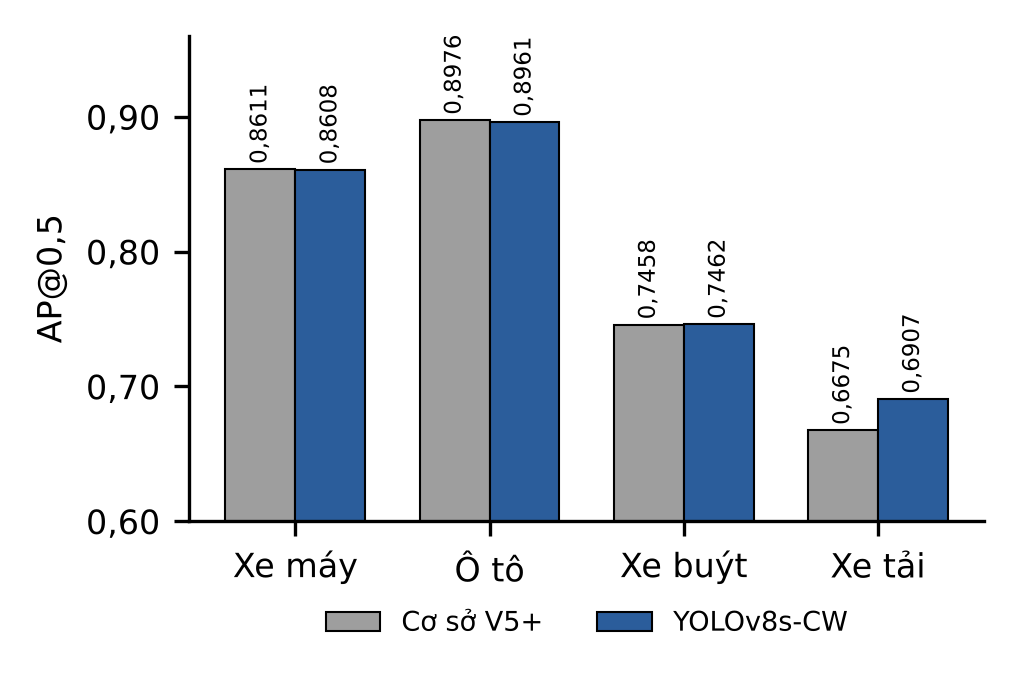
\includegraphics[width=\columnwidth]{fig2_ap_per_class.png}
\caption{AP@0,5 theo lớp của cơ sở V5+ và YOLOv8s-CW trên tập kiểm thử V5+. Thay đổi đáng kể duy nhất là ở xe tải.}
\label{fig:perclass}
\end{figure}

\subsection{Đánh giá ngoài miền trên VN Aerial}
Bảng~\ref{tab:aerial} cho thấy khoảng cách giữa trong miền và ngoài miền vẫn lớn: YOLOv8s-CW kém 19,66 điểm khi chuyển từ tập kiểm thử V5+ sang VN Aerial. So với cơ sở V5+, mức cải thiện của YOLOv8s-CW chỉ là 1,68 điểm trên VN Aerial xác thực và 0,22 điểm trên VN Aerial kiểm thử; ở thí nghiệm đối chứng, trung bình ba hạt giống trên VN Aerial kiểm thử là 0,6142 ($\clspw = 0{,}5$) và 0,6100 ($\clspw = 0$). Cấu hình p4\_scale đạt kết quả ngoài miền tốt nhất (0,6374 trên VN Aerial kiểm thử, tăng 3,78 điểm so với cơ sở), dù thấp hơn cơ sở trong miền. Như vậy không có một cấu hình nào tốt nhất ở mọi bối cảnh. YOLOv8s COCO không huấn luyện lại đạt 0,4893 trên VN Aerial kiểm thử. Kết quả ngoài miền của Faster R-CNN được báo cáo ở Bảng~\ref{tab:coco} vì được tính bằng pycocotools.

\begin{table}[!t]
\centering
\caption{mAP@0,5 trong miền và ngoài miền (VN Aerial) theo Ultralytics; chênh lệch là V5+ kiểm thử trừ Aerial kiểm thử, tính bằng điểm}
\label{tab:aerial}
\resizebox{\columnwidth}{!}{%
\begin{tabular}{lcccc}
\toprule
Mô hình & V5+ kiểm thử & Aerial xác thực & Aerial kiểm thử & Chênh lệch\\
\midrule
Cơ sở V5+ & 0,7930 & 0,6200 & 0,5996 & 19,34\\
p4\_scale & 0,7871 & 0,6476 & 0,6374 & 14,97\\
p4\_imgsz1280 & 0,7741 & 0,6377 & 0,6008 & 17,33\\
r\_p2 & 0,7528 & 0,5525 & 0,5380 & 21,48\\
r\_progressive & 0,7710 & 0,6287 & 0,6100 & 16,10\\
YOLOv8s-CW & 0,7984 & 0,6368 & 0,6018 & 19,66\\
$\clspw = 0$ (TB 3 lần) & 0,8003 & 0,6307 & 0,6100 & 19,03\\
$\clspw = 0{,}5$ (TB 3 lần) & 0,8008 & 0,6323 & 0,6142 & 18,66\\
YOLOv8s COCO & 0,4514 & -- & 0,4893 & --\\
\bottomrule
\end{tabular}}
\end{table}

\subsection{Phân tích lỗi}
Bảng~\ref{tab:errors} liệt kê số TP, FP, FN của YOLOv8s-CW. Xe tải có precision và recall thấp nhất (0,6593 và 0,6315); xe buýt có recall 0,6574. Xe máy có 10.206 FN, phần lớn do vật nhỏ: recall của xe máy là 49,8\% ở nhóm nhỏ, 79,3\% ở nhóm vừa và 95,4\% ở nhóm lớn; xe tải chỉ đạt 48,2\% ở nhóm vừa so với 86,1\% ở nhóm lớn. Nhầm lớp chủ yếu xảy ra giữa ô tô và xe buýt (207 trường hợp hai chiều), ô tô và xe tải (135) và xe buýt và xe tải (103); xe máy ít bị nhầm lớp (47 trường hợp) (Hình~\ref{fig:confusion}). Tập kiểm thử chỉ có ảnh ban ngày nên chúng tôi không kết luận về điều kiện ban đêm.

\begin{table}[!t]
\centering
\caption{TP, FP, FN theo lớp của YOLOv8s-CW (ngưỡng tin cậy 0,25; IoU ghép 0,5)}
\label{tab:errors}
\begin{tabular}{lrrrcc}
\toprule
Lớp & TP & FP & FN & P & R\\
\midrule
Xe máy & 29.517 & 4.290 & 10.206 & 0,8731 & 0,7431\\
Ô tô & 7.241 & 2.751 & 777 & 0,7247 & 0,9031\\
Xe buýt & 497 & 148 & 259 & 0,7705 & 0,6574\\
Xe tải & 538 & 278 & 314 & 0,6593 & 0,6315\\
\bottomrule
\end{tabular}
\end{table}

\begin{figure}[!t]
\centering
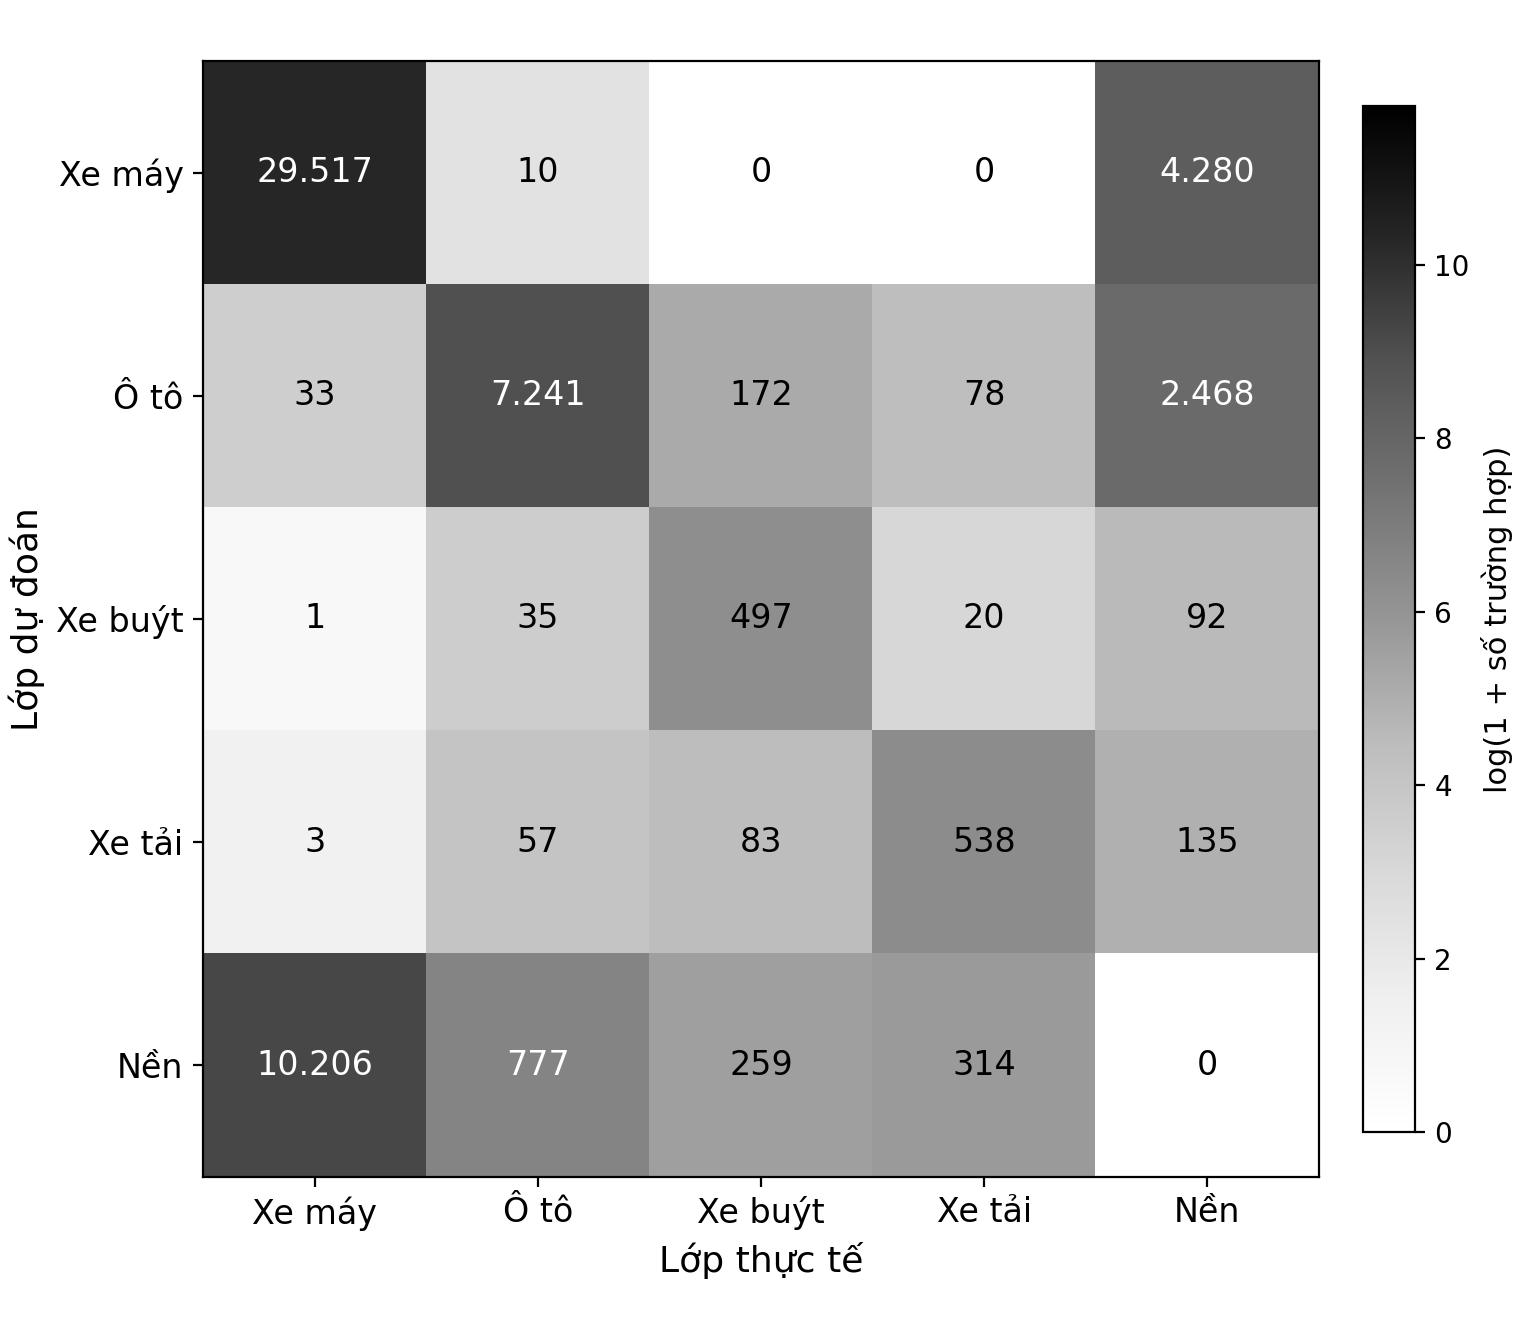
\includegraphics[width=0.9\columnwidth]{fig3_confusion.png}
\caption{Ma trận nhầm lẫn của YOLOv8s-CW trên tập kiểm thử V5+ (ngưỡng tin cậy 0,25; IoU ghép 0,5); hàng là lớp dự đoán, cột là lớp thực tế; độ đậm theo $\log(1 + \text{số trường hợp})$.}
\label{fig:confusion}
\end{figure}

\subsection{Tốc độ}\label{sec:speed}
Trên cùng GPU, trong cùng một phiên đo, với batch 1, 20 ảnh khởi động và 200 ảnh kiểm thử, độ trễ mỗi ảnh của YOLOv8s-CW (đầu vào 960) là 9,00~ms ở FP16 (trung vị 8,79~ms, phân vị 95 là 10,48~ms) và 9,75~ms ở FP32 (trung vị 9,52~ms); Faster R-CNN (cạnh ngắn 800, cạnh dài tối đa 1.333, FP32) mất 47,66~ms (trung vị 47,33~ms, phân vị 95 là 50,89~ms). Ở cùng FP32, YOLOv8s nhanh hơn khoảng 4,9 lần. Giữa các phiên đo khác nhau, độ trễ tuyệt đối của cả hai mô hình dao động tới khoảng 20--30\% theo trạng thái GPU, nên chúng tôi chỉ so sánh tỷ lệ đo trong cùng phiên. Phạm vi đo không hoàn toàn giống nhau: thời gian của YOLO gồm đọc và giải mã ảnh, tiền xử lý, suy luận và NMS; thời gian của Faster R-CNN gồm tiền xử lý bên trong mô hình (đổi kích thước, chuẩn hóa), suy luận và NMS nhưng không gồm đọc ảnh. Vì YOLO bị tính thêm phần đọc ảnh, tỷ lệ này không thiên vị YOLO. Khi ghép với ByteTrack và vạch đếm ảo, toàn bộ quy trình trên một video 178 khung hình ($1764 \times 948$ pixel) đạt 77,1 khung hình/giây khi không ghi video và 41,8 khung hình/giây khi ghi video đầu ra (đã khởi động trước).

\subsection{Kết quả đếm phương tiện}
Chúng tôi chưa đánh giá được độ chính xác của phép đếm. Video dùng để đo tốc độ ở Mục~\ref{sec:speed} là một đoạn 5,9 giây (30 khung hình/giây) quay đường cao tốc ở nước ngoài, không phải giao thông Việt Nam, và số lượt đếm tham chiếu của nó chỉ là ước lượng cho kiểm thử chức năng chứ không phải nhãn đếm tay. Vì vậy chúng tôi chỉ dùng video này để kiểm tra quy trình chạy đúng và đo tốc độ. Đánh giá phép đếm cần các video camera Việt Nam có nhãn đếm tay độc lập; chúng tôi cũng chưa có nhãn ID theo thời gian nên chưa đánh giá được bộ theo vết bằng IDF1 hay MOTA.

% ============================================================
\section{Thảo luận}
\textbf{Điều kết quả ủng hộ.} Thứ nhất, khi huấn luyện trên cùng dữ liệu và đánh giá bằng cùng công cụ, hai bộ phát hiện thể hiện một đánh đổi rõ: Faster R-CNN chính xác hơn trong miền (4,03 điểm mAP@0,5 so với YOLOv8s-CW), còn YOLOv8s nhanh hơn khoảng 4,9 lần ở cùng FP32 và nhỏ hơn khoảng 3,7 lần về số tham số. Theo pycocotools, AP@0,5 của Faster R-CNN là 0,8725, 0,8775, 0,7467 và 0,6696 (xe máy, ô tô, xe buýt, xe tải), so với 0,8454, 0,8855, 0,6476 và 0,6266 của YOLOv8s-CW: Faster R-CNN hơn ở xe máy, xe buýt, xe tải, chênh lớn nhất ở xe buýt, còn hai mô hình ngang nhau ở ô tô. Thứ hai, ngoài miền thứ tự đảo lại ở mAP@0,5 (YOLOv8s-CW cao hơn trên VN Aerial) nhưng không đảo ở mAP@0,5:0,95, và khoảng cách giữa trong miền và ngoài miền rất lớn với cả hai mô hình. Trong các cấu hình YOLO, các mô hình tinh chỉnh thêm từ cơ sở tốt nhất trong miền còn p4\_scale tốt nhất ngoài miền. Do đó chọn mô hình chỉ theo một tập kiểm thử có thể gây hiểu lầm. Thứ ba, trọng số lớp chỉ đóng góp rất ít: theo pycocotools, trung bình ba hạt giống của $\clspw = 0{,}5$ hơn $\clspw = 0$ là 0,13 điểm, chênh lệch theo từng hạt giống từ $-0{,}04$ đến +0,29 điểm, trong khi riêng việc tinh chỉnh thêm đã hơn cơ sở 1,12 điểm ([+0,75; +1,51]). Kết quả này phù hợp với quan sát của Crasto~\cite{crasto} trên YOLOv5 rằng đặt lại trọng số không mang lại hiệu quả tương xứng cho bộ phát hiện một giai đoạn.

\textbf{Điều kết quả chưa chứng minh.} Chúng tôi lưu ý bảy điểm để người đọc không diễn giải quá mức.
\begin{enumerate}
\item \textbf{Số lần huấn luyện.} Chỉ thí nghiệm trọng số lớp được lặp với ba hạt giống; ở đó độ lệch giữa các hạt giống là 0,3--0,4 điểm. Các cấu hình YOLO khác chỉ chạy một lần, nên chênh lệch dưới khoảng một điểm giữa chúng chưa đủ để xếp hạng. Khoảng tin cậy bootstrap chỉ phản ánh việc chọn ảnh kiểm thử.
\item \textbf{Mô hình cuối khác lịch học với đối chứng.} YOLOv8s-CW dùng lịch 15 epoch có dừng sớm, còn các lượt đối chứng dùng lịch 10 epoch. Chúng tôi giữ YOLOv8s-CW làm mô hình cuối cho các phân tích khác (lỗi, tốc độ, ngoài miền), nhưng kết luận về trọng số lớp dựa trên thí nghiệm đối chứng.
\item \textbf{Khác biệt giữa hai công cụ đánh giá.} Cùng một điểm lưu YOLO cho mAP@0,5 theo Ultralytics cao hơn theo pycocotools khoảng 4,7 điểm (0,7984 so với 0,7513 cho YOLOv8s-CW), do khác cách ghép dự đoán với nhãn và cách nội suy. Vì vậy con số của hai công cụ không được so trực tiếp với nhau, và kết quả của các công trình khác chỉ so được khi biết công cụ đánh giá.
\item \textbf{Chọn cấu hình đã tham khảo tập kiểm thử.} Việc chọn YOLOv8s-CW làm mô hình cuối có tham khảo kết quả trên tập kiểm thử và VN Aerial, nên đó là lựa chọn hậu nghiệm, và VN Aerial cũng không còn là tập chưa nhìn thấy hoàn toàn. Tập kiểm thử không cập nhật trọng số nhưng đã tham gia quyết định cấu hình.
\item \textbf{Hai mô hình khác cỡ và chưa được tinh chỉnh ngang nhau.} Faster R-CNN ResNet50-FPN có 41,4 triệu tham số, gấp khoảng 3,7 lần YOLOv8s, nên phần chênh độ chính xác một phần đến từ dung lượng mô hình chứ không chỉ từ kiến trúc hai giai đoạn. Faster R-CNN chỉ có một lượt huấn luyện 8 epoch với một hạt giống, trên GPU khác (Tesla T4), và điểm lưu tốt nhất rơi vào epoch cuối, nên ngân sách dài hơn có thể còn cải thiện; nhánh YOLO thì được thử nhiều cấu hình hơn. So sánh với một biến thể Faster R-CNN gọn hơn (ví dụ backbone MobileNetV3) hoặc một YOLOv8 lớn hơn sẽ cho bức tranh cùng cỡ đầy đủ hơn.
\item \textbf{Ngân sách huấn luyện không đều giữa các cấu hình YOLO.} Các cấu hình khởi tạo ấm (p4\_scale, p4\_imgsz1280, YOLOv8s-CW) được huấn luyện thêm trên nền cơ sở, còn r\_p2 và r\_progressive khởi tạo từ COCO với 25 và 30 epoch, ít hơn 40 epoch của cơ sở (Bảng~\ref{tab:config}). Vì vậy kết quả âm tính của P2 và lộ trình độ phân giải có thể một phần do thiếu ngân sách huấn luyện.
\item \textbf{Phạm vi dữ liệu hẹp.} Tập kiểm thử chỉ có hai camera ban ngày ở TP.HCM, VN Aerial chỉ có 635 ảnh một kiểu góc nhìn, tập xác thực chung khung cảnh với tập huấn luyện (Mục~\ref{sec:data}), và phép đếm chưa được đánh giá trên video Việt Nam có nhãn.
\end{enumerate}

\textbf{Kết quả âm tính.} Đầu phát hiện P2 giảm AP xe tải 12,27 điểm; tăng độ phân giải lên 1.280 giảm mAP 1,89 điểm; lộ trình độ phân giải giảm 2,20 điểm. Thí nghiệm nhãn giả dùng 402 khung hình lấy cách nhau 50 khung từ một video camera giao thông công khai (bộ \texttt{vn\_cctv\_traffic} trên Roboflow Universe); nhãn được sinh bằng YOLOv8s huấn luyện trên 2.833 ảnh nhãn thật của V5, chỉ giữ hộp có độ tin cậy từ 0,75 trở lên. Hai lượt YOLOv8s cùng cấu hình (khởi tạo COCO, ảnh 960, batch 16, tốc độ học 0,005, hạt giống 42) cho thấy thêm 402 ảnh nhãn giả vào 2.833 ảnh nhãn thật làm mAP@0,5 trên tập kiểm thử giảm từ 0,7812 xuống 0,7608 (2,04 điểm). Lượt không có nhãn giả chỉ ghi nhận 26/40 epoch trong nhật ký, còn lượt có nhãn giả chạy đủ 40 epoch, và nhãn giả chỉ đến từ một video, nên kết quả này chỉ cho thấy cách sinh nhãn giả trên không giúp ích trong thí nghiệm của chúng tôi. Chúng tôi báo cáo các kết quả âm tính vì chúng cho thấy các cải tiến trực giác không tự động có hiệu quả trên dữ liệu này, trong giới hạn ngân sách huấn luyện đã nêu ở điểm 6.

% ============================================================
\section{Kết luận}
Chúng tôi trình bày một đánh giá bộ phát hiện phương tiện giao thông Việt Nam trên bộ V5+ gồm 10.203 ảnh bốn lớp, chia tập theo video. Việc chia theo video chỉ giảm thiểu rò rỉ: toàn bộ 1.466 ảnh xác thực chung khung cảnh với tập huấn luyện, trong khi hai camera kiểm thử không xuất hiện trong huấn luyện. Khi huấn luyện trên cùng tập và đánh giá bằng cùng công cụ, Faster R-CNN ResNet50-FPN đạt mAP@0,5 là 0,7916 trên tập kiểm thử, cao hơn YOLOv8s-CW (0,7513) 4,03 điểm, còn YOLOv8s nhanh hơn khoảng 4,9 lần ở cùng FP32 với số tham số ít hơn khoảng 3,7 lần. Trên VN Aerial, YOLOv8s-CW có mAP@0,5 cao hơn (0,5991 và 0,5759 so với 0,5640 và 0,5242 trên tập xác thực và kiểm thử) nhưng Faster R-CNN có mAP@0,5:0,95 cao hơn; chênh lệch mAP@0,5 trên tập kiểm thử 149 ảnh chưa có ý nghĩa thống kê. Lựa chọn giữa hai mô hình vì vậy phụ thuộc vào yêu cầu tốc độ và bối cảnh triển khai. Trọng số lớp chỉ tạo khác biệt không đáng kể (dưới 0,3 điểm) khi so với đối chứng cùng quá trình tinh chỉnh; đầu phát hiện P2, tăng độ phân giải, lộ trình độ phân giải và việc thêm nhãn giả cũng không cải thiện kết quả trong miền. Do phần lớn cấu hình chỉ được huấn luyện một lần, hai mô hình được so khác cỡ, tập kiểm thử chỉ có hai camera ban ngày và tập xác thực còn rò rỉ, các kết luận là bằng chứng sơ bộ.

Hướng tiếp theo là: (i) chia lại dữ liệu theo khung cảnh camera (gộp ngày và đêm của cùng camera) và chọn cấu hình bằng tập xác thực độc lập; (ii) lặp lại các cấu hình YOLO còn lại với nhiều hạt giống; (iii) so sánh các mô hình cùng cỡ, ví dụ Faster R-CNN với backbone MobileNetV3 so với YOLOv8s, và YOLOv8 lớn hơn so với Faster R-CNN ResNet50-FPN, với nhiều hạt giống và ngân sách huấn luyện dài hơn; (iv) gán nhãn đếm tay cho video camera Việt Nam để đánh giá phép đếm và bộ theo vết; (v) mở rộng đánh giá ngoài miền sang camera ngang, ban đêm và nhiều địa phương.

% ------------------------------------------------------------
\section*{Lời cảm ơn}
Chúng tôi cảm ơn các nhóm tác giả đã phát hành công khai các bộ dữ liệu SOICT 2024, SOICT Night, Vehicle Vietnam-CanTho, Vietnamese Vehicle v3, Vietnam Vehicles v10 và VN Aerial được sử dụng trong nghiên cứu. Phần Abstract tiếng Anh và một số đoạn trong các Mục I--VII được biên tập với sự hỗ trợ của công cụ trí tuệ nhân tạo; các tác giả đã kiểm tra và chịu trách nhiệm về toàn bộ nội dung.

% ------------------------------------------------------------
\begin{thebibliography}{99}
\bibitem{yolo} J. Redmon, S. Divvala, R. Girshick, and A. Farhadi, ``You only look once: Unified, real-time object detection,'' in \textit{Proc. IEEE Conf. Comput. Vis. Pattern Recognit. (CVPR)}, 2016, pp. 779--788.
\bibitem{frcnn} S. Ren, K. He, R. Girshick, and J. Sun, ``Faster R-CNN: Towards real-time object detection with region proposal networks,'' in \textit{Proc. Adv. Neural Inf. Process. Syst. (NeurIPS)}, vol. 28, 2015, pp. 91--99.
\bibitem{trinh} T. Trinh and K. Nguyen, ``A Vietnamese benchmark for vehicle detection and real-time empirical evaluation,'' \textit{Can Tho Univ. J. Sci.}, vol. 14, no. 3, pp. 45--52, 2022, doi: 10.22144/ctu.jen.2022.042.
\bibitem{dinh} D.-L. Dinh, H.-N. Nguyen, H.-T. Thai, and K.-H. Le, ``Towards AI-based traffic counting system with edge computing,'' \textit{J. Adv. Transp.}, vol. 2021, Art. no. 5551976, 2021, doi: 10.1155/2021/5551976.
\bibitem{vuong} X. C. Vuong, R.-F. Mou, and T. T. Vu, ``Vehicle tracking and speed estimation under mixed traffic conditions using YOLOv4 and SORT: A case study of Hanoi,'' \textit{Transport Problems}, vol. 17, no. 4, pp. 17--26, 2022, doi: 10.20858/tp.2022.17.4.02.
\bibitem{resnet} K. He, X. Zhang, S. Ren, and J. Sun, ``Deep residual learning for image recognition,'' in \textit{Proc. IEEE Conf. Comput. Vis. Pattern Recognit. (CVPR)}, 2016, pp. 770--778.
\bibitem{fpn} T.-Y. Lin, P. Doll\'ar, R. Girshick, K. He, B. Hariharan, and S. Belongie, ``Feature pyramid networks for object detection,'' in \textit{Proc. IEEE Conf. Comput. Vis. Pattern Recognit. (CVPR)}, 2017, pp. 2117--2125.
\bibitem{ssd} W. Liu \textit{et al.}, ``SSD: Single shot multibox detector,'' in \textit{Proc. Eur. Conf. Comput. Vis. (ECCV)}, 2016, pp. 21--37.
\bibitem{ultra} Ultralytics, ``Explore Ultralytics YOLOv8,'' Ultralytics Docs. Accessed: Oct. 15, 2026. [Online]. Available: \url{https://docs.ultralytics.com/models/yolov8/}
\bibitem{gfl} X. Li \textit{et al.}, ``Generalized focal loss: Learning qualified and distributed bounding boxes for dense object detection,'' in \textit{Proc. Adv. Neural Inf. Process. Syst. (NeurIPS)}, vol. 33, 2020, pp. 21002--21012.
\bibitem{cbloss} Y. Cui, M. Jia, T.-Y. Lin, Y. Song, and S. Belongie, ``Class-balanced loss based on effective number of samples,'' in \textit{Proc. IEEE/CVF Conf. Comput. Vis. Pattern Recognit. (CVPR)}, 2019, pp. 9268--9277.
\bibitem{focal} T.-Y. Lin, P. Goyal, R. Girshick, K. He, and P. Doll\'ar, ``Focal loss for dense object detection,'' in \textit{Proc. IEEE Int. Conf. Comput. Vis. (ICCV)}, 2017, pp. 2980--2988.
\bibitem{eql} J. Tan \textit{et al.}, ``Equalization loss for long-tailed object recognition,'' in \textit{Proc. IEEE/CVF Conf. Comput. Vis. Pattern Recognit. (CVPR)}, 2020, pp. 11662--11671.
\bibitem{seesaw} J. Wang \textit{et al.}, ``Seesaw loss for long-tailed instance segmentation,'' in \textit{Proc. IEEE/CVF Conf. Comput. Vis. Pattern Recognit. (CVPR)}, 2021, pp. 9695--9704.
\bibitem{phan} T. H. Phan and K. Yamamoto, ``Resolving class imbalance in object detection with weighted cross entropy losses,'' 2020, arXiv:2006.01413.
\bibitem{bdd} F. Yu \textit{et al.}, ``BDD100K: A diverse driving dataset for heterogeneous multitask learning,'' in \textit{Proc. IEEE/CVF Conf. Comput. Vis. Pattern Recognit. (CVPR)}, 2020, pp. 2636--2645.
\bibitem{crasto} N. Crasto, ``Class imbalance in object detection: An experimental diagnosis and study of mitigation strategies,'' 2024, arXiv:2403.07113.
\bibitem{detrac} L. Wen \textit{et al.}, ``UA-DETRAC: A new benchmark and protocol for multi-object detection and tracking,'' \textit{Comput. Vis. Image Understand.}, vol. 193, Apr. 2020, Art. no. 102907.
\bibitem{coco} T.-Y. Lin \textit{et al.}, ``Microsoft COCO: Common objects in context,'' in \textit{Proc. Eur. Conf. Comput. Vis. (ECCV)}, 2014, pp. 740--755.
\bibitem{mixup} H. Zhang, M. Cisse, Y. N. Dauphin, and D. Lopez-Paz, ``mixup: Beyond empirical risk minimization,'' in \textit{Proc. Int. Conf. Learn. Represent. (ICLR)}, 2018.
\bibitem{ultraloss} Ultralytics, ``Detection loss implementation,'' source code, v8.4.126. Accessed: Nov. 16, 2026. [Online]. Available: \url{https://github.com/ultralytics/ultralytics/blob/v8.4.126/ultralytics/utils/loss.py}
\bibitem{tv} TorchVision, ``fasterrcnn\_resnet50\_fpn,'' TorchVision Documentation. Accessed: Oct. 15, 2026. [Online]. Available: \url{https://docs.pytorch.org/vision/main/models/generated/torchvision.models.detection.fasterrcnn_resnet50_fpn.html}
\bibitem{bytetrack} Y. Zhang \textit{et al.}, ``ByteTrack: Multi-object tracking by associating every detection box,'' in \textit{Proc. Eur. Conf. Comput. Vis. (ECCV)}, 2022, pp. 1--21.
\end{thebibliography}

\end{document}
